\documentclass[tikz,border=3mm]{standalone}
\usetikzlibrary{arrows.meta, positioning, quotes}

\begin{document}
    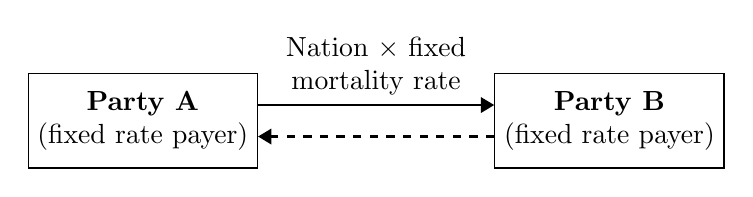
\begin{tikzpicture}[
    node distance=5mm and 30mm,
box/.style = {draw, minimum height=12mm, align=center},
sy+/.style = {yshift= 2mm}, 
sy-/.style = {yshift=-2mm},
every edge quotes/.style = {align=center}
                        ]
\node (n1) [box]             {\textbf{Party A}\\(fixed rate payer)};                        
\node (n2) [box,right=of n1] {\textbf{Party B}\\(fixed rate payer)};
%
\draw[thick,-Triangle]  
    ([sy+] n1.east) to [above,"Nation $\times$ fixed\\ mortality rate"] ([sy+] n2.west);
\draw[thick,-Triangle, dashed]  
    ([sy-] n2.west) -- ([sy-] n1.east);
    \end{tikzpicture}

    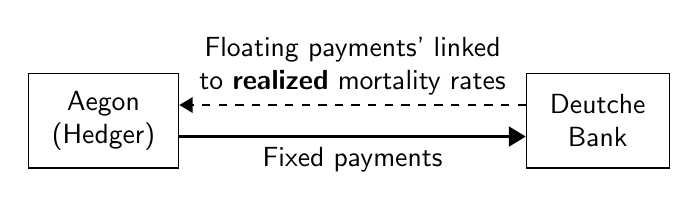
\begin{tikzpicture}[
    node distance=5mm and 44mm,
box/.style = {draw, minimum height=12mm, inner xsep=3mm, align=center},
sy+/.style = {yshift= 2mm},
sy-/.style = {yshift=-2mm},
every edge quotes/.style = {align=center},
     font = \sffamily
                        ]
\node (n1) [box]             {Aegon\\(Hedger)};
\node (n2) [box,right=of n1] {Deutche\\Bank};
%
\draw[thick,-Triangle, dashed]
    ([sy+] n2.west) to [above,"Floating payments' linked\\
                              to \textbf{realized} mortality rates"] ([sy+] n1.east);
\draw[very thick,-Triangle]
    ([sy-] n1.east) to[below,"Fixed payments"] ([sy-] n2.west);
    \end{tikzpicture}
\end{document}
